\documentclass[12pt]{article}
\usepackage{graphicx}
\usepackage[margin=1in]{geometry}
\usepackage{setspace}
\usepackage{booktabs}
\usepackage{hyperref}
\usepackage[
backend=biber,
style=alphabetic,
]{biblatex}
\addbibresource{references.bib}
\usepackage{amsmath} 


\title{Predicting the Housing Market using \\ Linear Regression}

\author{Garrick Ho\\
  Jun Yan\\[1ex]
  Department of Statistics\\
  University of Connecticut\\
}

\doublespacing
\begin{document}

\maketitle
\doublespace

\begin{abstract}
With the housing market fluctuating every year, many real estate owners and businesses face a problem with gaining an accurate representation of the future of the housing market. Lots of people do not know much about the market, so they will go to real estate owners or businesses to learn more about the market. And then see what the market is at and if it is the right time to buy a house. If real estate owners and businesses are able to gain more accuracy in predicting the housing market, they will be able to help more people and possibly gain more business. Not only can this benefit the consumers, the builders are able to move with the market and have a better understanding of it. This paper aims to construct a robust linear regression model by using machine learning techniques to predict housing costs accurately. By leveraging natural language processing, the linear regression model analyzes home property descriptions and extracts vital insights that significantly contribute to precise pricing predictions. This paper ends with an explanation of the limitations of this study and potential future works that can be done.

\bigskip
\noindent{\sc Keywords}:
housing market;
natural language processing;
linear regression;
model predictions


\end{abstract}

\section{Introduction}
\label{sec:intro}

% Why does it matter?
% What has already been done?
% What is new?

The United States has been through three recessions in the last decade. And during that decade, house prices have reached the very bottom of the market and also reached the very top of the market. The market has tripled since 1992. After a brief dip in 2002-2003, they bounced back and skyrocketed over 20\% from May 2003 to November 2004. \cite{Jacobsen2005} Because of the constant change, new models for predicting the housing market also need to change so that the model can stay up to date with the changes that occur. This is important because it gives people insights into whether it's a good time to buy or sell a property, helps policymakers make informed decisions, and allows investors to strategize their moves. House price predictions can help the developer determine the selling price of a house and can also help the customer arrange the right time to purchase a house. \cite{alfiyantin2017} 

Engineers in the past had to face a significant challenge in forecasting and assessing house prices. Fortunately, with technological advances, machine learning algorithms offer a solution, enabling users to predict house prices by training data sets on various algorithms. The market is currently flooded with software and models designed to enhance the accuracy of house price predictions, minimizing errors to negligible levels. These predictions can be based on the analysis of different aspects of a house, such as kitchen size, bedroom count, bathroom count, and overall land area. These aspects of a house can go on forever. Analysts employ various techniques to compute and analyze data,  to ensure that the predictions are aligned closely with previous estimations. \cite{singh2021}

Existing methods for predicting housing prices often rely on traditional statistical models that may struggle to capture the complexity and non-linear relationships present in real estate markets. Additionally, these models may not effectively incorporate the wide range of features that influence property values. An attractive solution would involve leveraging advanced machine learning techniques, such as multiple linear regression, to handle the complexity and non-linearity of the data. This allows the model to learn intricate patterns and relationships that may be challenging for traditional methods. Additionally, a comprehensive solution should consider factors such as location, economic indicators, property characteristics, and even social trends to build a more accurate and robust predictive model. The key is to strike a balance between model complexity and interpretability while ensuring it can effectively handle the diverse and dynamic nature of the real estate market.
% An overview of the topic
% Existing works
% Why are existing methods not sufficient? What are the elements of an attractive solution?
% Contributions
The main contribution of this paper is to corroborate the findings of prior research papers on this topic.

% A roadmap
The rest of the paper is organized in the following way. Beginning with the overall introduction located in Section~\ref{sec:intro}. A brief introduction about the data will be shown in Section~\ref{sec:data}. Here, the variables will be described and explained how they contribute to the research question. Then, the methodology used in this paper will be explained in Section~\ref{sec:meth}. The applications of the results found will be in Section~\ref{sec:app}. This section will present the results from the model and have further analysis with tables and figures. More in-depth analysis of how the results can be applied to the real world will be in this section. Finally, the discussion part for this paper will be in Section~\ref{sec:disc}. The limitations of the current study and future direction will be discussed here.



\section{Data}
\label{sec:data}

% Who collected the data (source)?
% How was the data collected? Sampling frame? Sampling approach?
% What period or range does the data cover?
% Why does the data help answer the research question?
% What exploratory analyses are done (descriptives, visualization, etc.)?

The data that will be used for this study was sourced from \href{https://www.kaggle.com/code/ashydv/housing-price-prediction-linear-regression/input}{Kaggle}. It is a data set that contains \(n = 545\) observations (different house samples) of thirteen variables, seven of which are categorical variables and six are numerical variables. The data set contains features and corresponding labels for training and testing a Multiple Linear Regression (MLR) model to predict the house cost.
The data was explored and visualized using the pandas library in Python. For the columns that were strings, they have been transformed into an integer data type so that they can be read in the model. More specifically, the 'furnishingstatus' column was broken down into three different columns. One for furnished, one for semi-furnished, and lastly one for unfurnished. 


\begin{table}
\caption{Data Description}
  \label{tab:rv}
\begin{tabular}{llll}
  \toprule
Variable & Data Type & Instance & Purpose \\
  \midrule
price & Int & 13300000 & \(Y\) \\ 
area & Int & 7420 & \(X_{n}\) \\ 
bedrooms & Int & 4 & \(X_{n}\) \\ 
bathrooms & Int & 2 & \(X_{n}\) \\ 
stories & Int & 3 & \(X_{n}\) \\ 
mainroad & Str & yes, no & \(X_{n}\) \\
guestroom & Str & yes, no & \(X_{n}\) \\
basement & Str & yes, no & \(X_{n}\) \\
hotwaterheating & Str & yes, no & \(X_{n}\) \\
airconditioning & Str & yes, no & \(X_{n}\) \\
parking & Int & 2 & \(X_{n}\) \\
prefarea & Str & yes, no & \(X_{n}\) \\
furnishingstatus & Str & furnished, semi-furnished, unfurnished & \(X_{n}\) \\
   \bottomrule
\end{tabular}\par
\bigskip
In Table~\ref{tab:rv}, the 'variable' column shows the names of all the variables that are in the dataset. The 'Data Type' column shows the data type of each variable in the dataset. Note that 'Int' means integer and 'Str' means string. The 'Instance' column shows an example of what a data point for that column would look like. The 'Purpose' column shows the importance of each variable to the machine learning step.
\end{table}

\begin{figure}
    \caption{Categorical Variable Plots}
    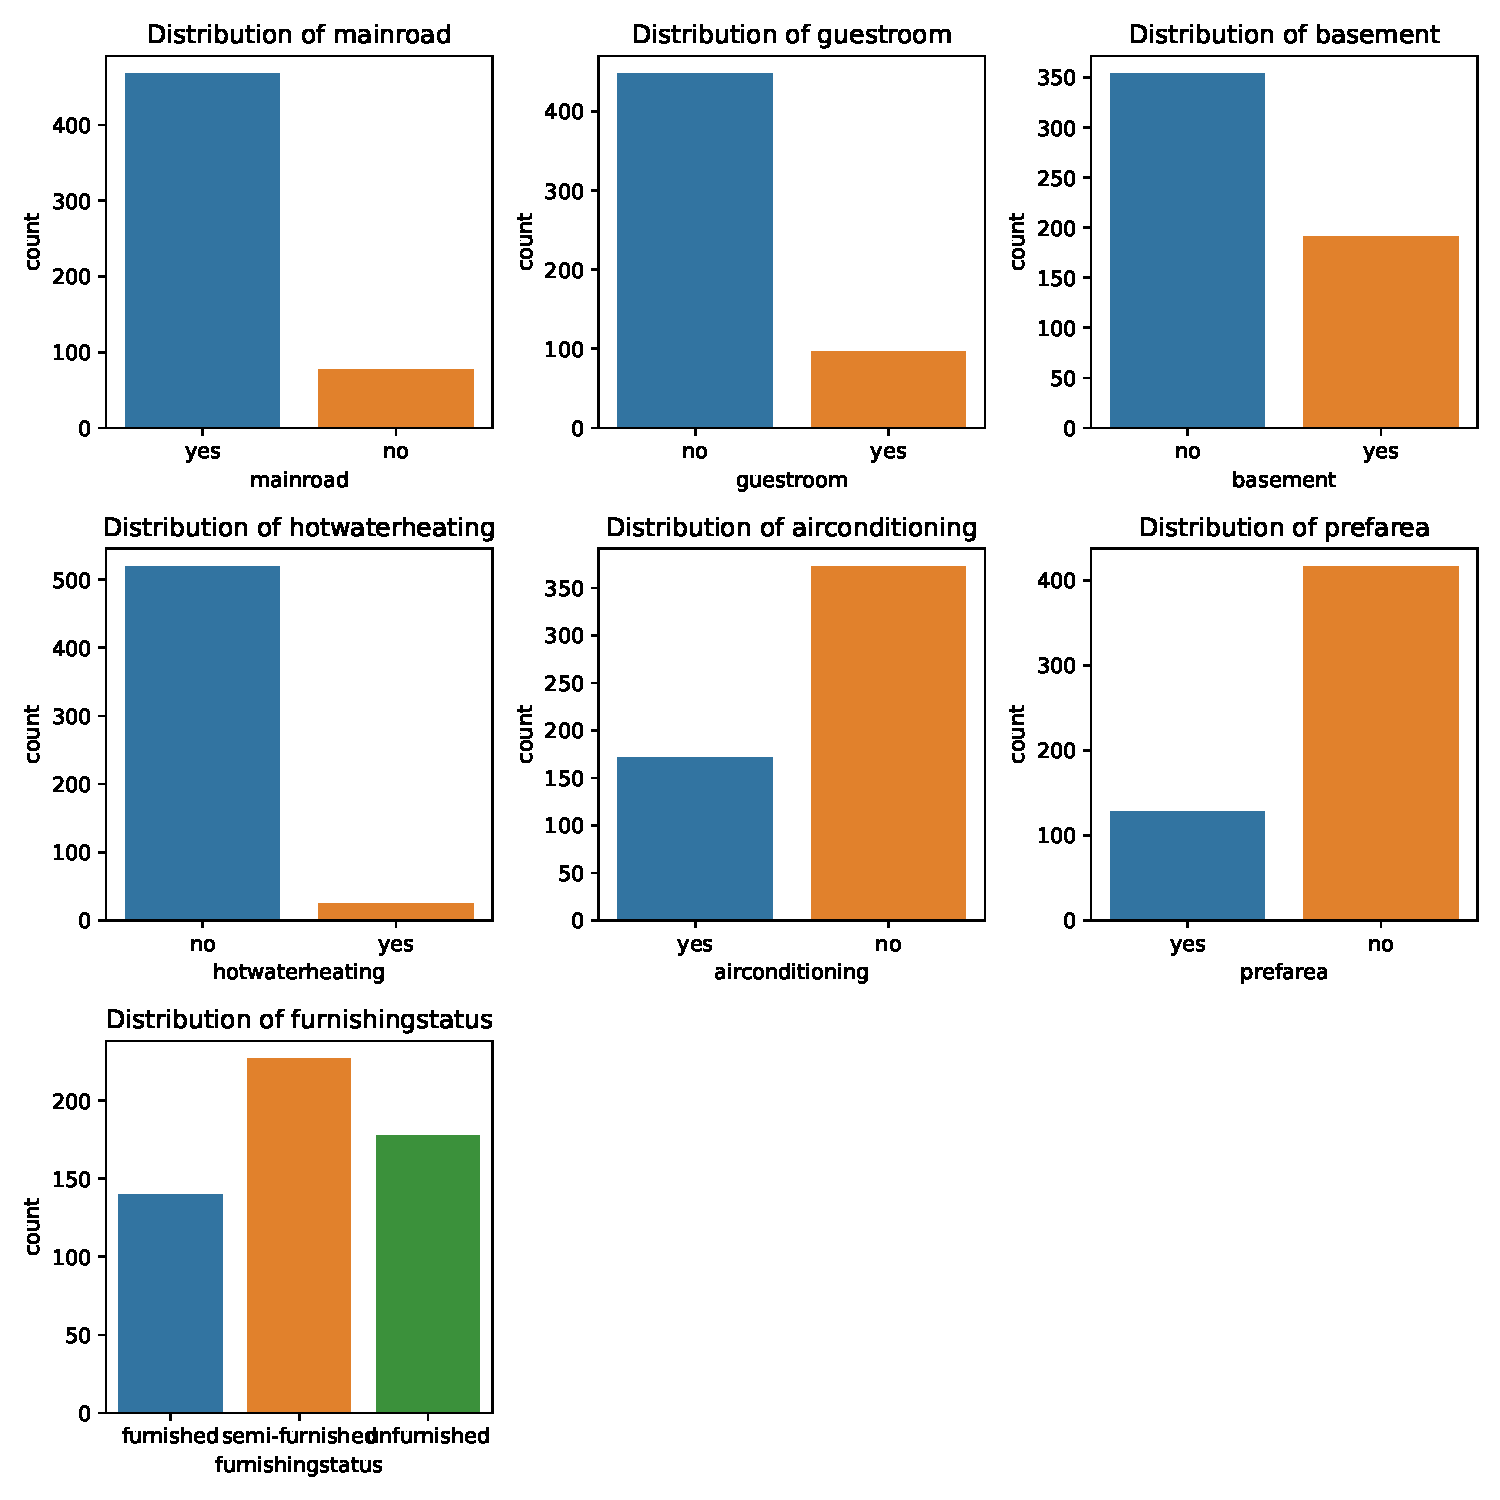
\includegraphics[width=1\textwidth]{categorical_plots.pdf}
    \label{fig:categorical_plots}
In figure~\ref{fig:categorical_plots}, the plots show the distributions for all the categorical variables. Most of the houses in this data set are located near a main road. Only one-fifth of the houses have a room for guests. For the basement category, two-fifths of them have one. Almost none of the houses have hot water heating. There is air conditioning in about two-fifths of the data. About one-fifth of the houses are located in a preferred area. And lastly, the house can come either furnished, semi-furnished, or unfurnished. Most of the house came semi-furnished, next being unfurnished and then fully furnished. 
\end{figure}

\begin{figure}
    \caption{Numerical Variable Plots}
    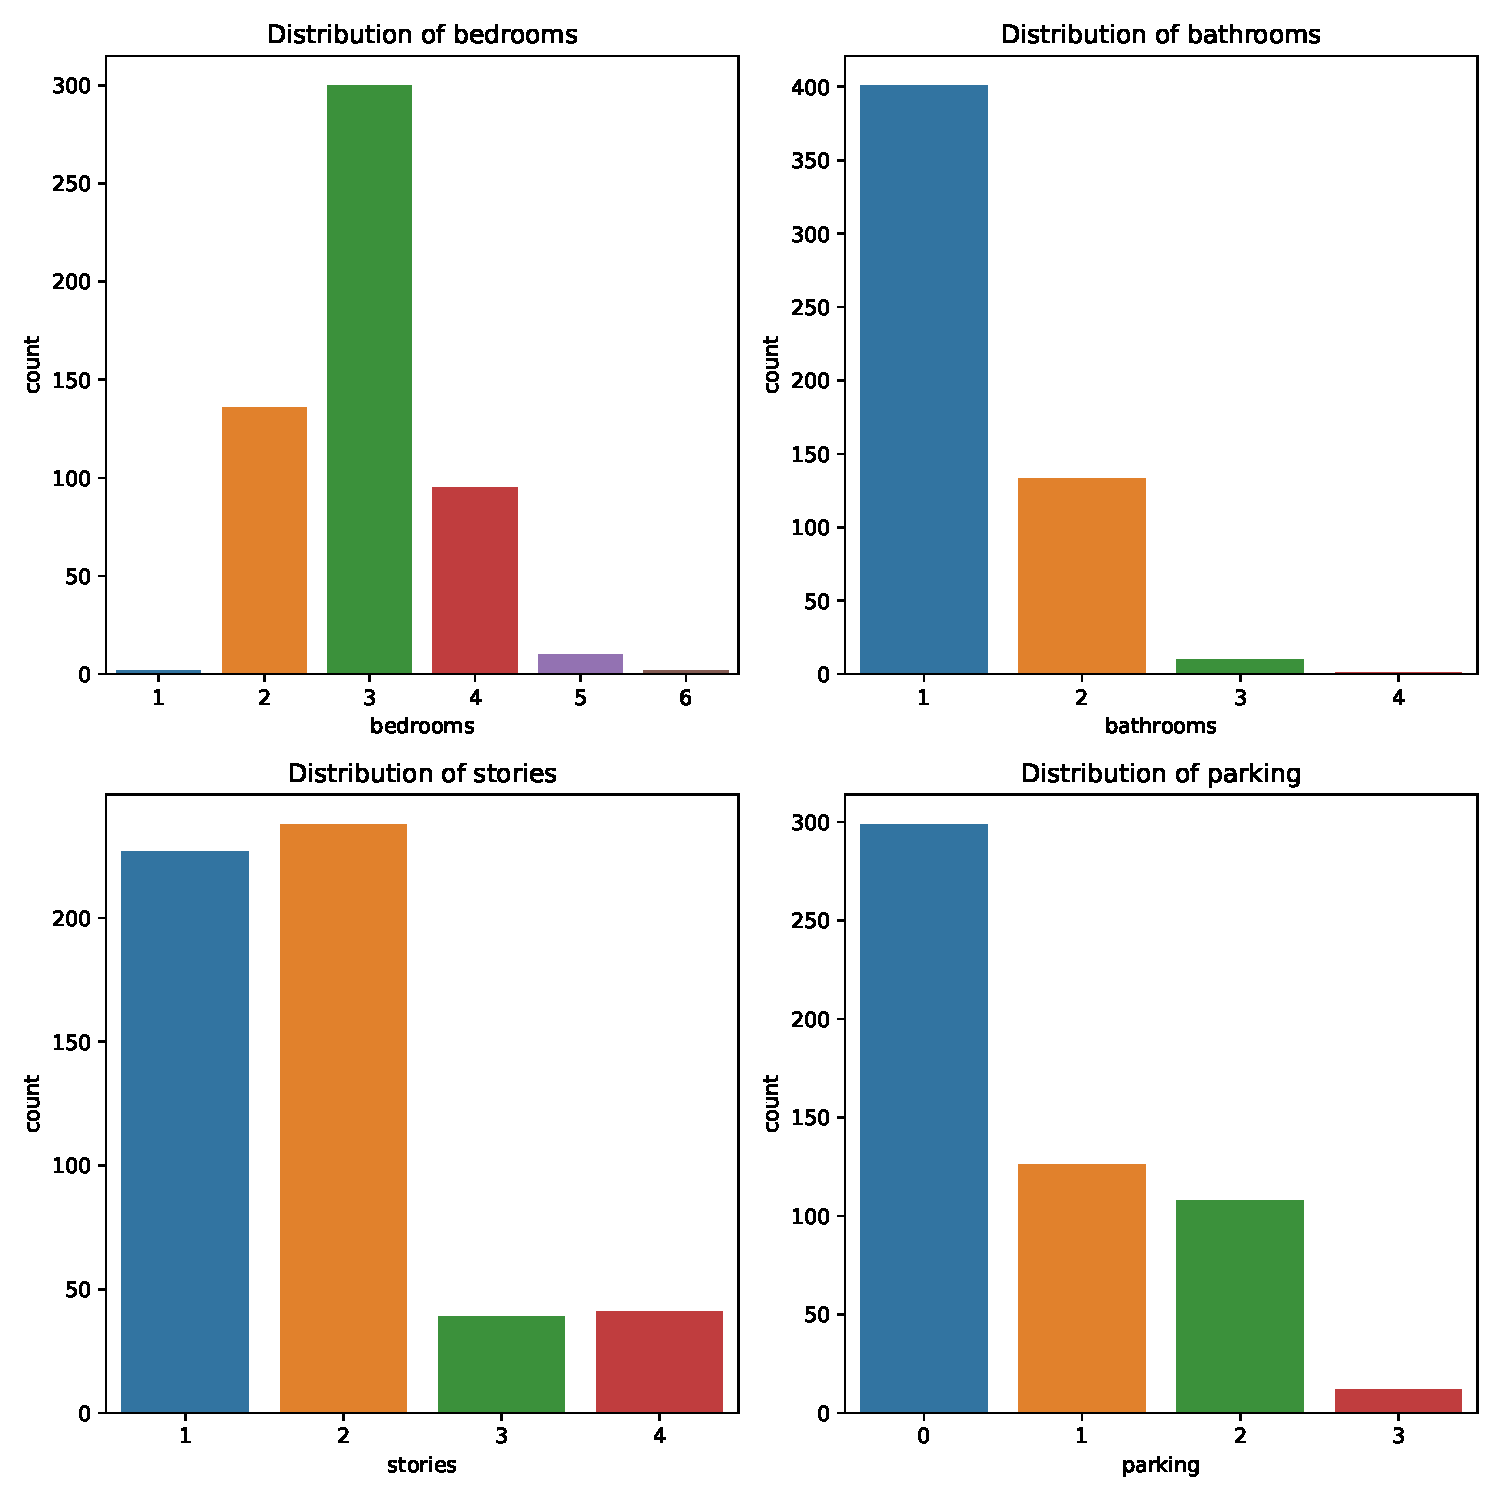
\includegraphics[width=1\textwidth]{numerical_plots.pdf}
    \label{fig:numberical_plots}
In figure~\ref{fig:numberical_plots}, four different plots are shown to display the distribution of the numerical variables in the data. The average number of bedrooms in these homes is three, with two being the second most. For the number of bathrooms, the majority of homes have one. About half of the homes in the data are one-story homes while about the other half are two stories. For parking, most of them have no parking spots. A few of them have one or two parking spots. 
\end{figure}

\section{Methods}
\label{sec:meth}

% Establish notation.
% What are the observed data?
% What are the models?
% What are the parameters to be estimated?
% How are the point estimators obtained?
% How are the uncertainty (standard errors) of the point estimators assessed?
% How are the variances of the point estimators estimated?
% How are the null distribution of the testing statistics established?
% Clearly state the assumptions and claims of theoretical results.
The data was first processed by making all the variables in the data able to be read by the model. The first variable that was altered was the status of the house being furnished. It was converted into dummy variables. A one in the dummy variable would mean that the house was in that current status and a zero would mean that it was not in that status. After that, the next step was to convert the yes and no entries to 1's and 0's. This was done to the variables mainroad, guestroom, basement, hotwaterheating, airconditioning, and prefarea. Before splitting the data set into training and testing groups, the variables were scaled because the values for price and the area of the house were significantly larger than the other values in the data set. Scaling is needed here because we want the values from each variable to contribute equally to the model and avoid the overpowering features with larger values. Finally, the data is split into \(80\%\) for training and 20\% for testing. The size of the training group was arbitrarily chosen to be greater than the size of the testing set to ensure that the multiple linear regression model is trained on as much data as possible to find and learn meaningful patterns. It is widely accepted for training data to be larger than testing data. An inadequate amount of training data can result in a poor-performing model that underfits and does not generalize to new instances well. A multiple linear regression model was fitted to the training group and then validated on the testing group using the scikit-learn library in Python. Several performance metrics about the predictions were then assessed.


\begin{equation}
  \label{eq:Multi}
  Y = \beta_{0} + \beta_{1}X_{1} + \beta_{2}X_{2} + ... + \beta_{n}X_{n} + \epsilon
\end{equation}

Equation~\ref{eq:Multi} is the Multiple Linear Regression model being used. \(Y\) is the dependent variable, also known as the value that is being predicted. In this case, it would be the cost of a house. \(X_{n}\) is the independent variable, which is the characteristics of the house that are used to predict the house cost. \(\beta_{n}\) is the average amount by which the dependent variable increases and decreases depending on when the independent variable increases one standard deviation. When all the other independent variables are held constant. \(\beta_{0}\) represents the value of the dependent variable when all the independent variables are equal to zero. \(\epsilon\) is the error term which represents the margin of error within the linear regression model. \cite{uyanik2013}



\section{Application}
\label{sec:app}

% Report the statistical analyses in tables/figures.
% When summarizing from tables/figures, paint the big picture, rather than reiterating all of the little details.
% Discussions to link the analyses 

This linear regression model aims to predict the house price with the different characteristics of a house by using the trained data and testing it against the testing data. To see how well the model performed in predicting the house prices, R-squared was used and a visualization was created to help see the results. The figure below represents how the model did with predicting the house prices. As we can see, there is a clear trend in the plot showing the accuracy of the model. One noticeable trend in the plot is that the model's predicted value of the house is undervalued compared to the actual price of the house. This trend with the model can be supported with the R-squared value.

\begin{align}
\label{eq:R2}
\begin{split}
    R^2 &= 1 - \frac{\text{sum squared regression (SSR)}}{\text{total sum of squares (SST)}}, \\
    &= 1-\frac{\sum(y_i - \hat{y_i})^2 }{\sum(y_i - \Bar{y})^2} 
\end{split}
\end{align}

Equation~\ref{eq:R2} is the formula for R-squared. R-squared is a measure of the goodness of fit of a model. The sum squared regression is the sum of the residuals squared and the total sum of squares is the sum of the distance the data is away from the mean all squared. It is a percentage that takes the values between 0 and 1. If the percentage is 1, then the variation in the \(y\) values is accounted for by the \(x\) values. If the percentage is 0, then none of the variations of the \(y\) values is accounted for by the \(x\) values. \cite{kasuya2018}

\begin{figure}[h!]
    \caption{Linear Regression Plot}
    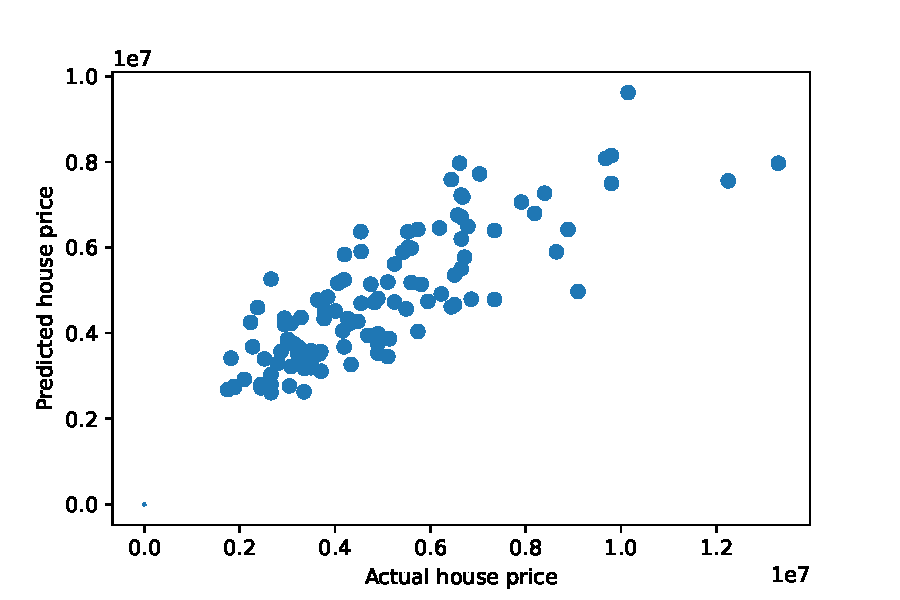
\includegraphics[width=1\textwidth]{linear_regression_plot.pdf}
    \label{fig:regression_plot}
\end{figure}
Figure~\ref{fig:regression_plot} shows a linear regression plot with the predicted house price against the actual house price. Based on this plot that was created, it looks like the model was somewhat accurate in predicting the prices. 

The calculated R-squared value for the model was 0.6529. An R-squared value of 0.6529 indicates the proportion of the variance in the dependent variable that can be explained by the independent variables in a multiple linear regression model. In other terms, about 65.29\% of the variability in the observed data can be accounted for by the model. 

\section{Discussion and Conclusion}
\label{sec:disc}

% A summary, again, of the contributions of the research.
% The research question posed as the `need’ of the introduction must be answered here (Zeiger 2000).
% Limitations of the current study
One limitation of this current study is that this data set is very small and has very limited variables. The next step for this study is to gain access to a data set from the actual house market and produce a model with it. Another factor that can limit this study is that nowadays, there are infinite numbers of factors that can affect the cost of a house. So creating a model to include all these new factors is practically impossible. 

% Future directions.
In the last decade, there have been three recessions in the United States. Being able to create a stronger model that can precisely predict the market can be more beneficial than just looking at house prices. If the model can see the fluctuation in the market, then the model can also help predict when the next recession is going to hit. 


% Every reference cited in the paper should appear here.
% References not cited should not appear here.
% All are automatically taken care of by BibTeX.
% Styles are controlled by bib style (.bst file).


\medskip

\printbibliography[title={References}]


\end{document}
